

% LaTeX file for Chapter Exp3




\chapter{Experiment 3: ITE model robustness in RCTs (simulation)} \label{ch:experiment3}




\section{Motivation}

In this section, we perform a simulation study to estimate the ITE using different models in an RCT setting under various scenarios. The aim is to identify conditions under which ITE estimation fails, and whether such failure is model-agnostic -- i.e., driven by external factors such as unobserved covariates or the strength of the treatment effect, rather than by the model class itself. This may provide insight into why ITE estimation can fail in real-world applications, as demonstrated by \citet{chen2025} on the IST dataset and replicated in our own work in Experiment 2 (Section~\ref{sec:results_experiment2}). 


\section{Setup} \label{sec:methods_experiment3}

The simulation is based on a data-generating process (DGP) that resembles an RCT. We assume a binary outcome and a set of covariates that influence the outcome. There may also be treatment-covariate interactions that are responsible for heterogeneity in the treatment effect.

\medskip

\textbf{Data-generating process:} Data is generated similarly to the approach proposed by \citet{hoogland2021}. The binary treatment ($T$) is sampled from a Bernoulli distribution with probability 0.5. The five covariates ($\mathbf{X}$), representing patient-specific characteristics at baseline, are drawn from a multivariate standard normal distribution with a compound symmetric covariance matrix ($\rho=0.1$). The binary outcome ($Y$) is sampled from a Bernoulli distribution with probability $\text{P}(Y_i = 1 \mid  \mathbf{X_i} = \mathbf{x_i}, T_i = t_i) = \text{logit}^{-1} \left(\beta_0 + \beta_T t_i + \boldsymbol{\beta}_X^\top \mathbf{x_i} + t_i \cdot \boldsymbol{\beta}_{TX}^\top \mathbf{x_{TX,i}} \right)$, where $i$ denotes the patient index, and $\mathbf{x}_{TX,i}$ denotes the subset of covariates that interact with the treatment.

The simulated datasets are generated under three scenarios, where coefficients are set to different values or not all variables are observed. In Scenario 1, the coefficients are: $\beta_0 = 0.45$ (intercept), $\beta_T = -0.85$ (direct treatment effect), $\boldsymbol{\beta}_X = (-0.5, 0.8, 0.2, 0.6, -0.4)$ (direct covariate effects), and $\boldsymbol{\beta}_{TX} = (0.9, 0.1)$ (interaction effects between treatment and covariates $X_1$ and $X_2$ on the outcome). In Scenario 2, the same coefficients are used, but the covariate $X_1$, which is responsible for a large portion of the heterogeneity, is not observed in the final dataset. This is expected to cause difficulties in estimating the ITE. In Scenario 3, the coefficients for the direct treatment and interaction effects are set to $\beta_T = -0.05$ and $\boldsymbol{\beta}_{TX} = (-0.01, 0.03)$ to represent a weak treatment effect and low heterogeneity. All other coefficients remain unchanged, and all covariates are observed. The DAGs corresponding to the three scenarios are presented in Figure~\ref{fig:simulation_dags}.


% here include 3 figures side by side 
% /img/results_ITE_simulation/simulation_observed.png
% simulation_unobserved.png
% simulation_small_effects.png

\begin{figure}[H]
\centering
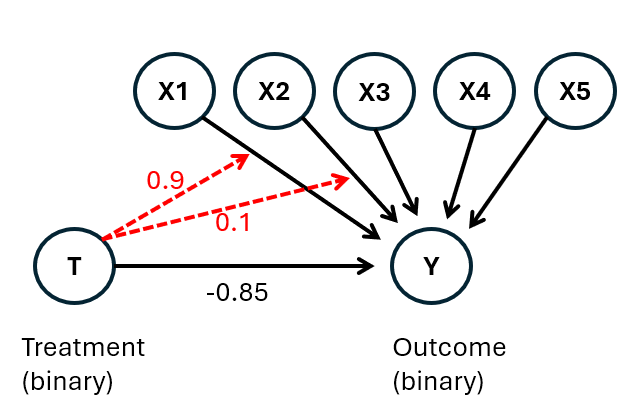
\includegraphics[width=0.3\textwidth]{img/results_ITE_simulation/simulation_observed.png}
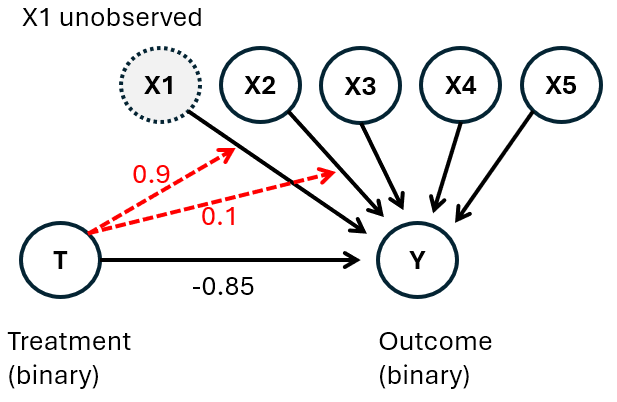
\includegraphics[width=0.3\textwidth]{img/results_ITE_simulation/simulation_unobserved.png}
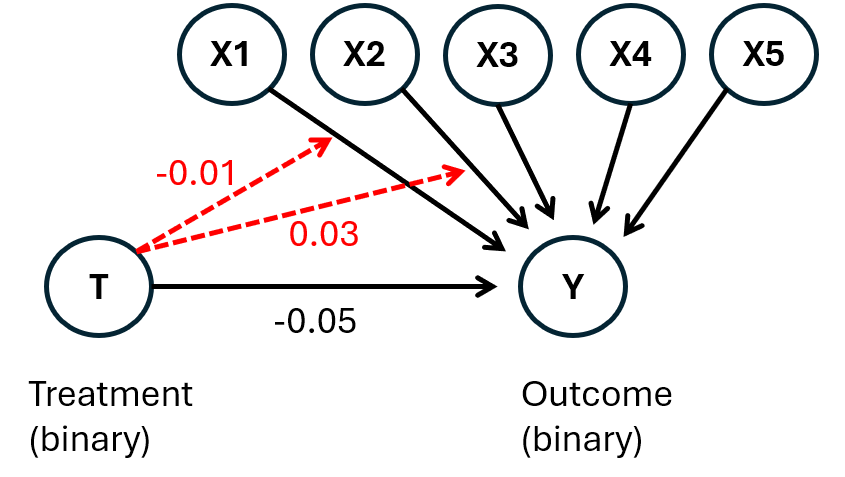
\includegraphics[width=0.3\textwidth]{img/results_ITE_simulation/simulation_small_effects.png}
\caption{Data-generating process (DGP) for the three scenarios in the ITE simulation study (RCT). Interaction effects between treatment ($T$) and covariates ($X_1$ and $X_2$) on the outcome ($Y$) are shown in red. Left: Scenario 1, where all covariates are observed and both treatment effect and heterogeneity are strong; Middle: Scenario 2, with the same DGP as in Scenario 1, but where covariate $X_1$ is not observed; Right: Scenario 3, where the treatment effect and heterogeneity are weak, and all covariates are observed.}
\label{fig:simulation_dags}
\end{figure}




% The data is generated for three different scenarios, where the coefficients are set to different values to represent different treatment effects and interaction effects and by removing the covariate $X1$ from the final dataset in scenario 2, hence making it unobserved. The scenarios are summarized in Table \ref{tab:simulation_scenarios}.


% Table with szenarios:

% Szenario 1: 
% description: strong direct and interaction effect of treatment, fully observed
% coefficients: \beta_0 = 0.45, \beta_T = -0.85,  \boldsymbol{\beta}_X = c(-0.5, 0.8, 0.2, 0.6, -0.4), \boldsymbol{\beta}_{TX} = c(0.9, 0.1)
% motivation: this scenario should represent the ideal case where there is high heterogeneity and all variables are observed, hence the ITE estimation is assumed to work well.

% Szenario 2:
% description: strong direct and interaction effect of treatment, but covariate X1 not observed
% coefficients: \beta_0 = 0.45, \beta_T = -0.85,  \boldsymbol{\beta}_X = c(-0.5, 0.8, 0.2, 0.6, -0.4), \boldsymbol{\beta}_{TX} = c(0.9, 0.1)
% motivation: removing the covariate X1, which is responsible for much of the heterogeneity, should cause difficulties in ITE estimation because the heterogeneity can not be attributed to the right covariate.

% Szenario 3:
% description: weak direct and interaction effect of treatment, fully observed
% coefficients: \beta_0 = 0.45, \beta_T = -0.05,  \boldsymbol{\beta}_X = c(-0.5, 0.8, 0.2, 0.6, -0.4), \boldsymbol{\beta}_{TX} = c(-0.01, 0.03)
% motivation: this scenario should represent the case where the treatment effect is weak and heterogeneity is low, hence the model should estimate only small range of ITE.





% \subsubsection*{Scenario 1: Strong effects, all covariates observed}
% 
% This scenario represents an ideal case in which the treatment has a strong direct and interaction effect. All covariates are observed, supposedly enabling effective ITE estimation. The coefficients are set as follows:
% 
% 
% 
% % X1 and X2 interact with treatment
% \begin{align*}
%     \beta_0 &= 0.45,\quad \beta_T = -0.85, \\
%     \boldsymbol{\beta}_X &= (-0.5,\ 0.8,\ 0.2,\ 0.6,\ -0.4), \\
%     \boldsymbol{\beta}_{TX} &= (0.9,\ 0.1) , X_1 \text{ and } X_2 \text{ interact with treatment}
% \end{align*}
% 
% \vspace{0.5em}
% 
% \subsubsection*{Scenario 2: Strong effects, covariate \boldmath$X_1$ unobserved}
% 
% This scenario uses the same coefficients as Scenario 1, but with covariate $X_1$ removed from the dataset. As $X_1$ drives a large portion of the treatment effect heterogeneity, the estimation of the ITE is expected to be biased or incomplete when $X_1$ is not observed.
% 
% 
% \begin{align*}
%     \beta_0 &= 0.45,\quad \beta_T = -0.85, \\
%     \boldsymbol{\beta}_X &= (-0.5,\ 0.8,\ 0.2,\ 0.6,\ -0.4), \\
%     \boldsymbol{\beta}_{TX} &= (0.9,\ 0.1) , X_1 \text{ and } X_2 \text{ interact with treatment}
% \end{align*}
% \textit{Note: $X_1$ is not included in the final dataset.}
% 
% \vspace{0.5em}
% 
% \subsubsection*{Scenario 3: Weak Effects, All Covariates Observed}
% 
% This scenario illustrates a setting with minimal treatment effect and weak treatment-covariate interaction. While all covariates are observed, the model is expected to recover only low-variance ITEs due to limited signal.
% 
% \begin{align*}
%     \beta_0 &= 0.45,\quad \beta_T = -0.05, \\
%     \boldsymbol{\beta}_X &= (-0.5,\ 0.8,\ 0.2,\ 0.6,\ -0.4), \\
%     \boldsymbol{\beta}_{TX} &= (-0.01,\ 0.03), X_1 \text{ and } X_2 \text{ (weakly) interact with treatment}
% \end{align*}


\textbf{Models for ITE estimation:} We applied the following models in \texttt{R} to estimate individualized treatment effects (ITEs): T-learner logistic regression (\texttt{stats} package), T-learner and S-learner logistic lasso regression (\texttt{glmnet} package \citep{friedman2010}, with $\lambda$ selected via 10-fold cross-validation), T-learner random forest (\texttt{randomForest} package \citep{breiman2001}, 100 trees), and T-learner tuned random forest (\texttt{comets} package \citep{comets}, which tunes \texttt{mtry} and \texttt{max.depth} using out-of-bag error, 500 trees).

While all models were run, we focus on two for the main results: the T-learner logistic regression as a baseline (matching the DGP), and the tuned random forest as a more flexible non-parametric model. Results for the default random forest in Scenario 1 are shown in Appendix~\ref{sec:default_rf_ite} to highlight the role of model tuning in avoiding overfitting and ensuring proper calibration.

Each model was trained and evaluated on independent datasets of 10,000 samples generated from the same DGP. Although TRAM-DAGs are well suited for ITE estimation, we did not include them here, as the goal of this experiment is to compare simpler and more complex models under varying conditions. TRAM-DAGs are evaluated in other experiments in this thesis.
% 
% 
% \textbf{Models for ITE estimation:} We applied the following models in \texttt{R} to estimate the ITEs: T-learner logistic regression (\texttt{stats} package), T-learner logistic lasso regression (\texttt{glmnet} package \citep{friedman2010}, with the regularization parameter $\lambda$ estimated via 10-fold cross-validation), S-learner logistic lasso regression (same as the T-learner), T-learner random forest (\texttt{randomForest} package \citep{breiman2001}, 100 trees), and T-learner tuned random forest (\texttt{comets} package \citep{comets}, which tunes the number of variables considered for splitting at each node (\texttt{mtry}) and the maximum tree depth (\texttt{max.depth}) using out-of-bag error, 500 trees). 
% 
% While all models were applied, we present only the results of the T-learner logistic regression as a benchmark (same model as used in the data-generating process), and the tuned random forest as representation of a complex non-parametric model. In Appendix~\ref{sec:default_rf_ite}, we additionally present the results for a standard random forest evaluated for Scenario 1 to illustrate the importance of model tuning to prevent overfitting and ensure accurate calibration.
% 
% All models were trained on a training set and evaluated on a test set, each consisting of 10,000 samples generated from the same DGP. TRAM-DAGs would also be well suited for ITE estimation in this setting, but we chose not to apply them in this experiment, since the main objective is to assess behavioral differences between complex and simple models under different scenarios. TRAM-DAGs are applied in other experiments in this thesis.

\medskip

\textbf{Model evaluation:} Model performance is evaluated visually on both the training and test datasets. For predictive performance, we present true vs. predicted probabilities $\text{P}(Y = 1 \mid X, T)$ to assess how well each model is calibrated. Plots of true vs. predicted ITEs show how closely the model estimates match the true effects. Since the true probabilities and ITEs are known by design in this simulation, direct evaluation of calibration and prediction accuracy is possible, unlike in real-world applications.

To assess whether estimated ITEs correspond to actual observed outcomes, we use ITE-ATE plots. These show the observed average treatment effect (ATE), calculated as $\text{P}(Y = 1 \mid T = 1) - \text{P}(Y = 1 \mid T = 0)$, in the respective subgroups of estimated ITEs. Accurate models should produce ITE-ATE points that align with the identity line.

These simulation scenarios allow us to assess ITE estimation performance under challenging conditions such as omitted variables and weak treatment effects. The subsequent results reveal which models remain robust under such violations and provide insight into possible real-world estimation failures.




\section{Results} \label{sec:results_experiment3}

In this section, we present the performance of two causal machine learning models -- T-learner logistic regression and T-learner tuned random forest -- for estimating ITEs under the three simulated scenarios introduced in Section~\ref{sec:methods_experiment3}. Scenario~(1) represents the ideal case where all covariates are observed and both treatment and interaction effects are strong. In Scenario~(2), a key effect modifier is unobserved, and in Scenario~(3), treatment and interaction effects are weak, but all covariates are observed.

Results for all scenarios are presented in Figures~\ref{fig:fully_observed_glm_tlearner} to~\ref{fig:small_interaction_tuned_rf_tlearner}.



\subsection{Scenario (1): Fully observed, large effects}



\begin{figure}[htbp]
\centering
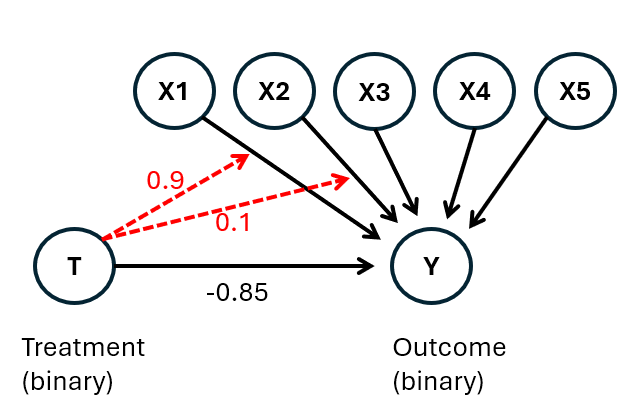
\includegraphics[width=0.35\textwidth]{img/results_ITE_simulation/simulation_observed.png}
\caption{DAG for Scenario~(1), where all variables are observed and both treatment and interaction effects are strong. This DAG was previously shown in Figure~\ref{fig:simulation_dags} and is re-plotted here for convenience. The numbers indicate the coefficients on the log-odds scale. Red arrows represent interaction effects between treatment ($T$) and covariates ($X_1$ and $X_2$) on the outcome ($Y$).}
\label{fig:fully_observed_dag}
\end{figure}


\begin{figure}[htbp]
\centering
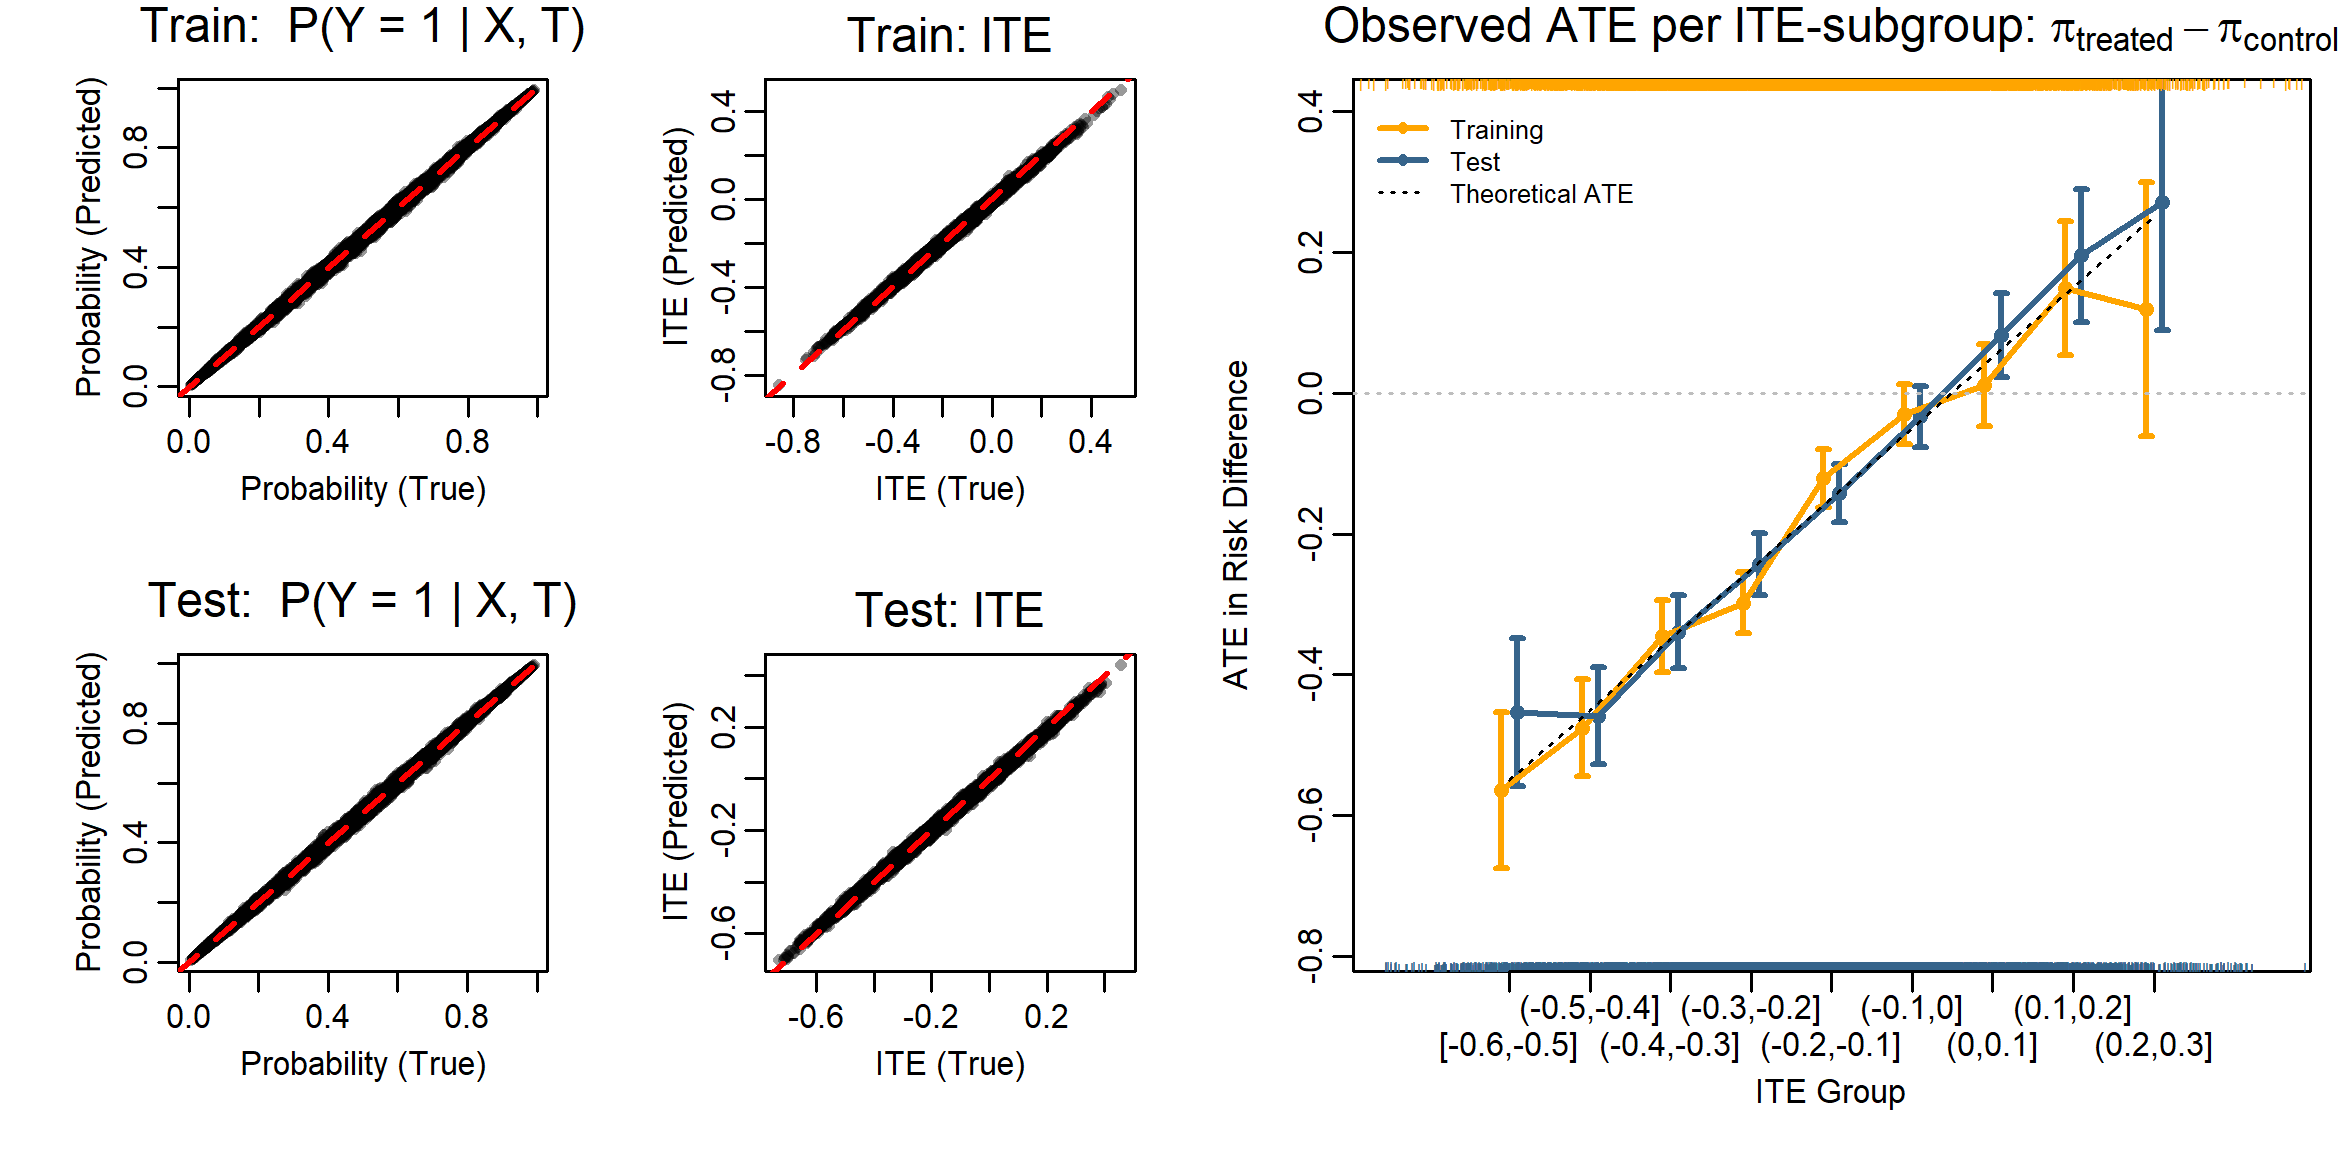
\includegraphics[width=0.9\textwidth]{img/results_ITE_simulation/fully_observed_glm_tlearner.png}
\caption{Results of the T-learner logistic regression in Scenario~(1), where the DAG is fully observed and both treatment and interaction effects are strong. Left: true vs. predicted probabilities for $\text{P}(Y = 1 \mid X, T)$; Middle: true vs. predicted ITEs; Right: observed ATE in terms of risk difference per estimated ITE subgroup.}
\label{fig:fully_observed_glm_tlearner}
\end{figure}


\begin{figure}[htbp]
\centering
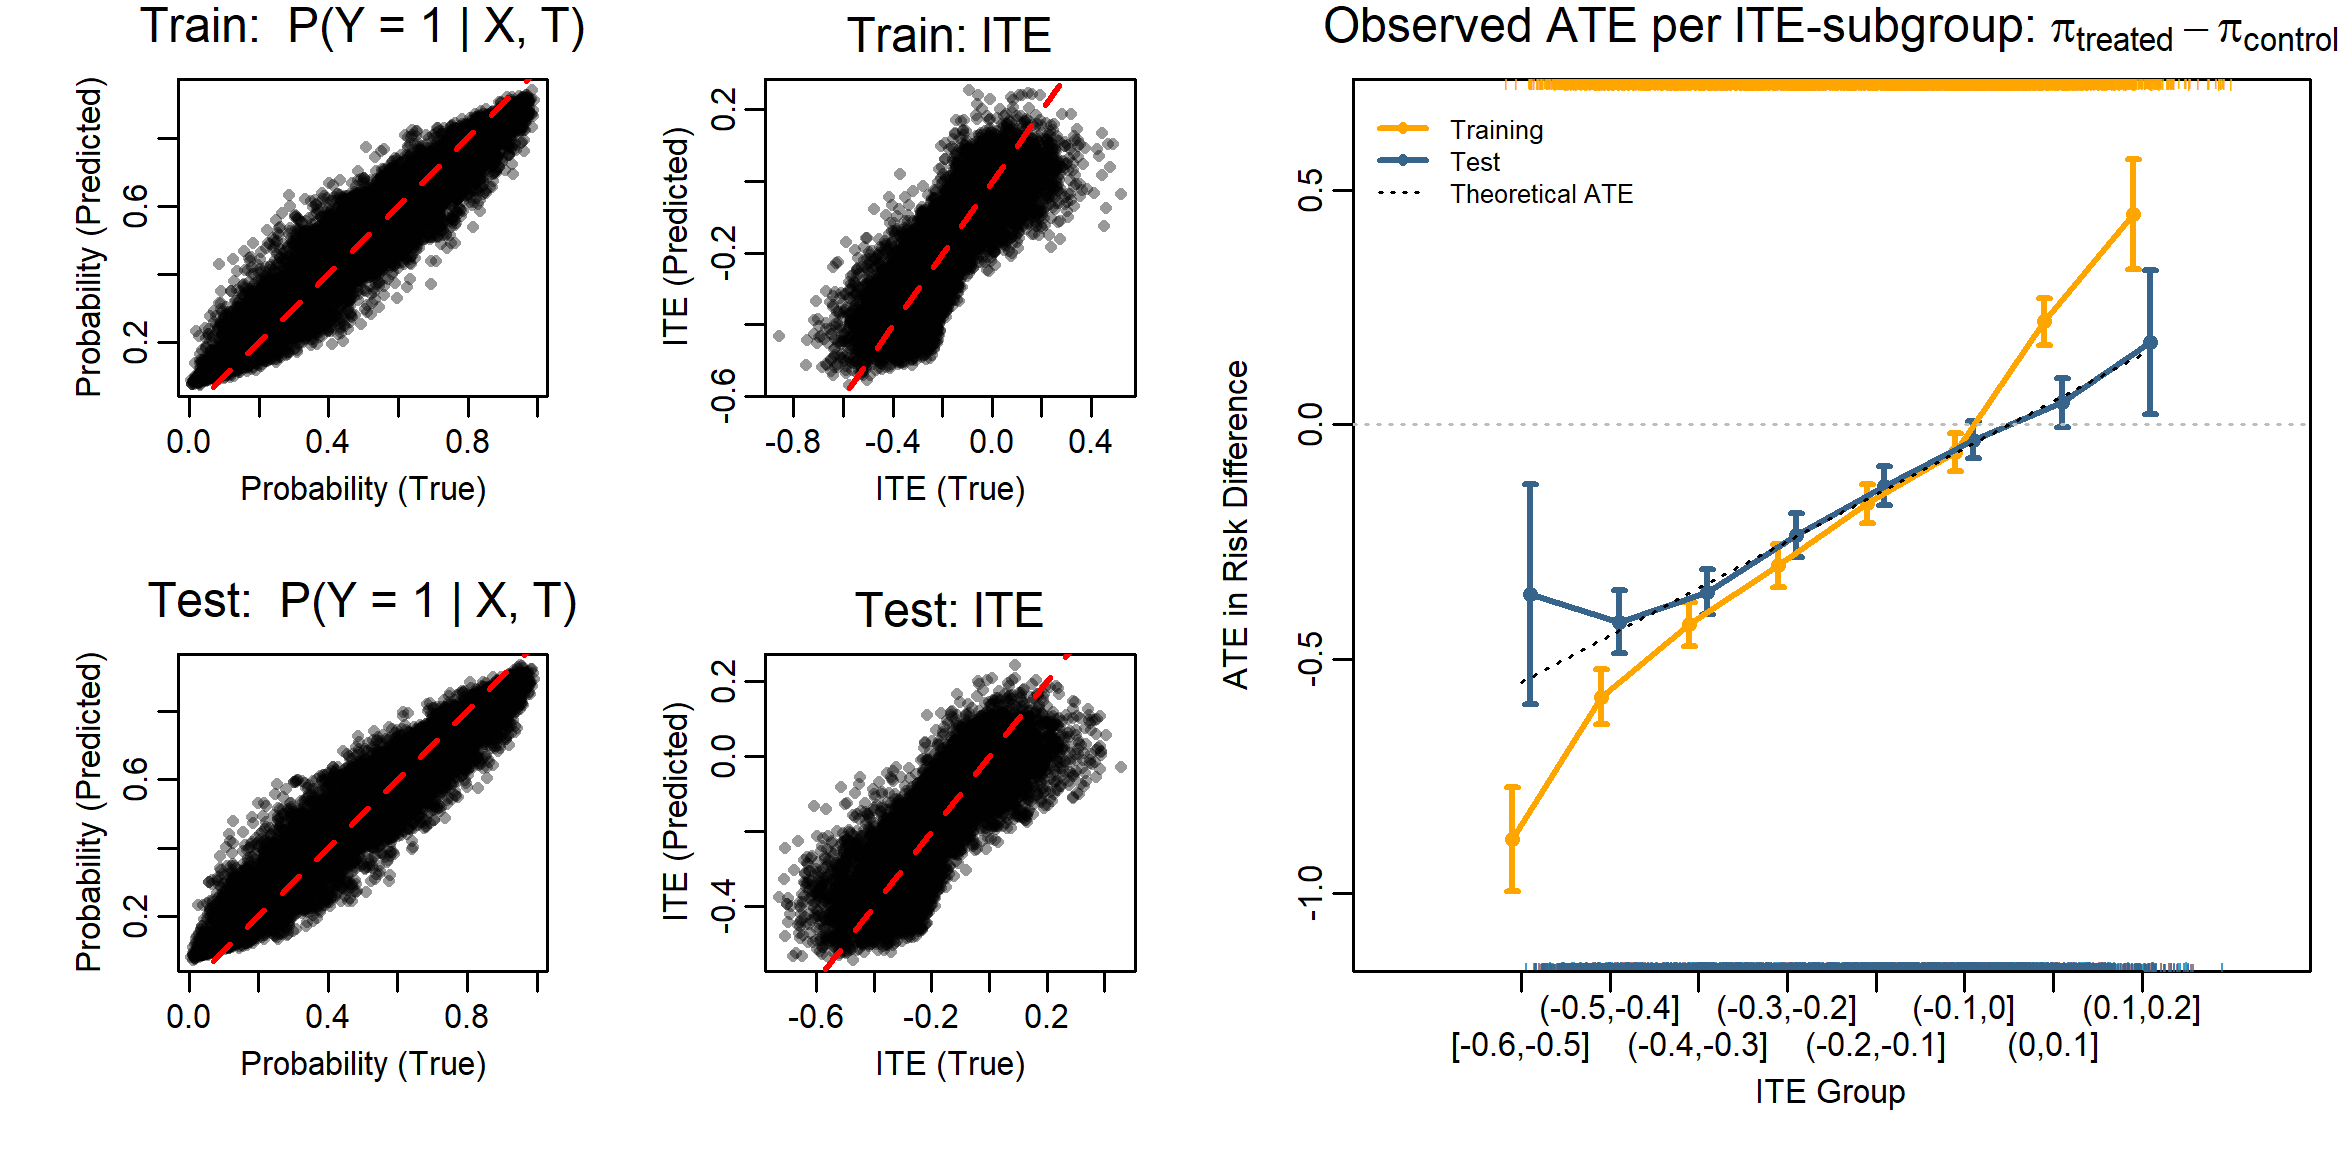
\includegraphics[width=0.9\textwidth]{img/results_ITE_simulation/fully_observed_tuned_rf_tlearner.png}
\caption{Results of the T-learner tuned random forest in Scenario~(1), where the DAG is fully observed and both treatment and interaction effects are strong. Left: true vs. predicted probabilities for $\text{P}(Y = 1 \mid X, T)$; Middle: true vs. predicted ITEs; Right: observed ATE in terms of risk difference per estimated ITE subgroup.}
\label{fig:fully_tuned_rf_tlearner}
\end{figure}


\clearpage



\subsection{Scenario (2): Unobserved interaction}

\begin{figure}[htbp]
\centering
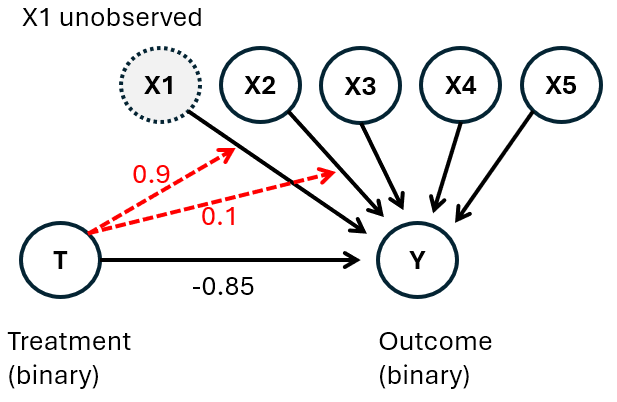
\includegraphics[width=0.35\textwidth]{img/results_ITE_simulation/simulation_unobserved.png}
\caption{DAG for Scenario~(2), where there are strong treatment and interaction effects, but variable $X_1$ is not observed. This DAG was previously shown in Figure~\ref{fig:simulation_dags} and is re-plotted here for convenience. The numbers indicate the coefficients on the log-odds scale. Red arrows represent interaction effects between treatment ($T$) and covariates ($X_1$ and $X_2$) on the outcome ($Y$).}
\label{fig:unobserved_interaction_dag}
\end{figure}



\begin{figure}[htbp]
\centering
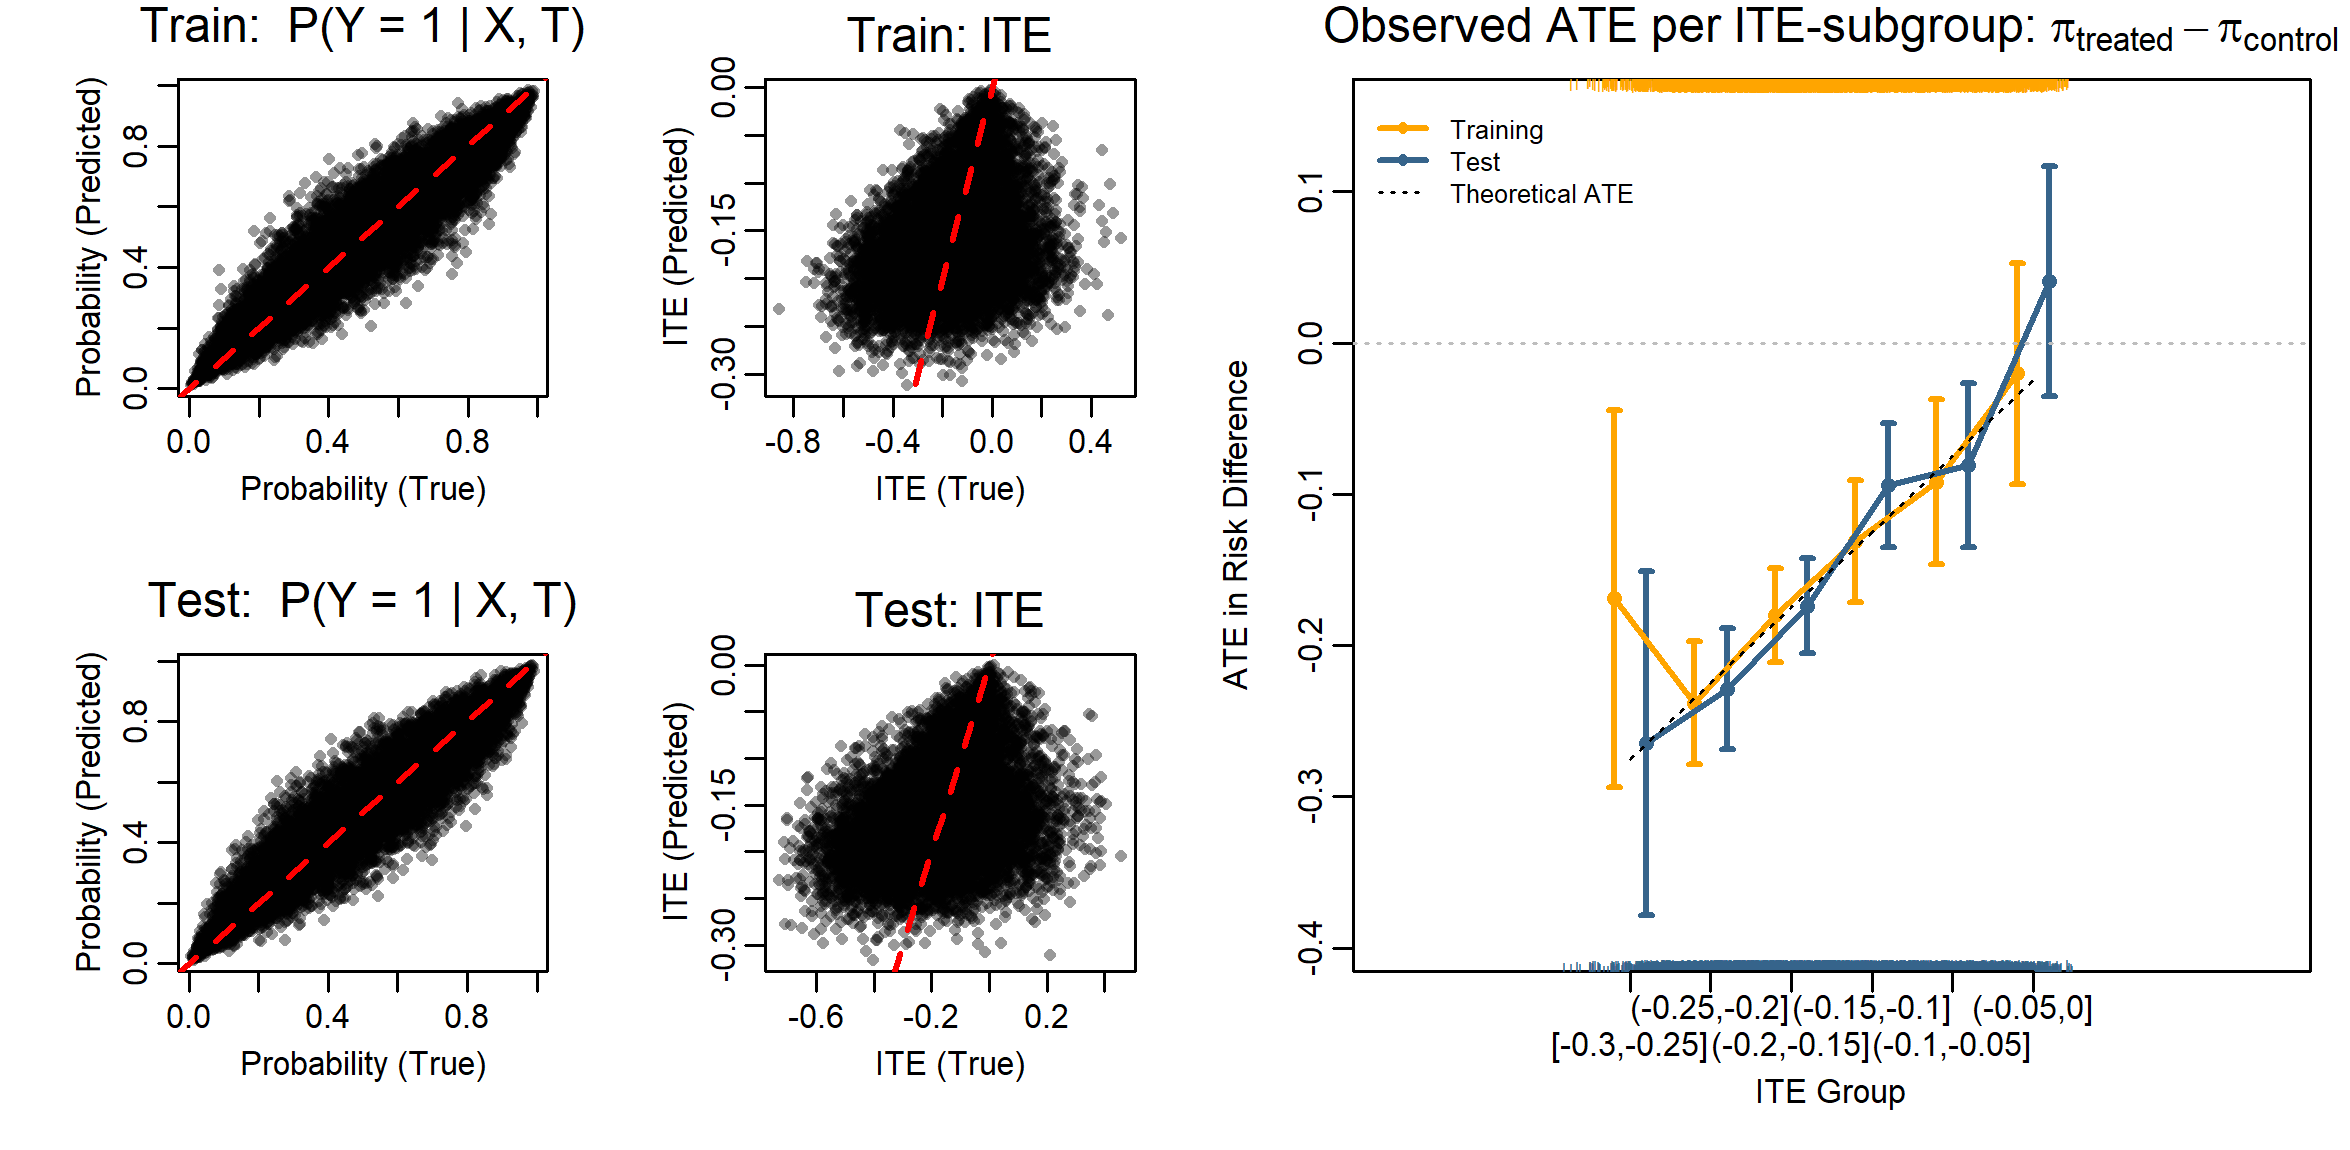
\includegraphics[width=0.9\textwidth]{img/results_ITE_simulation/unobserved_interaction_glm_tlearner.png}
\caption{Results of the T-learner logistic regression in Scenario~(2), where there are strong treatment and interaction effects, but variable $X_1$ is not observed. Left: true vs. predicted probabilities for $\text{P}(Y = 1 \mid X, T)$; Middle: true vs. predicted ITEs; Right: observed ATE in terms of risk difference per estimated ITE subgroup.}
\label{fig:unobserved_interaction_glm_tlearner}
\end{figure}



\begin{figure}[htbp]
\centering
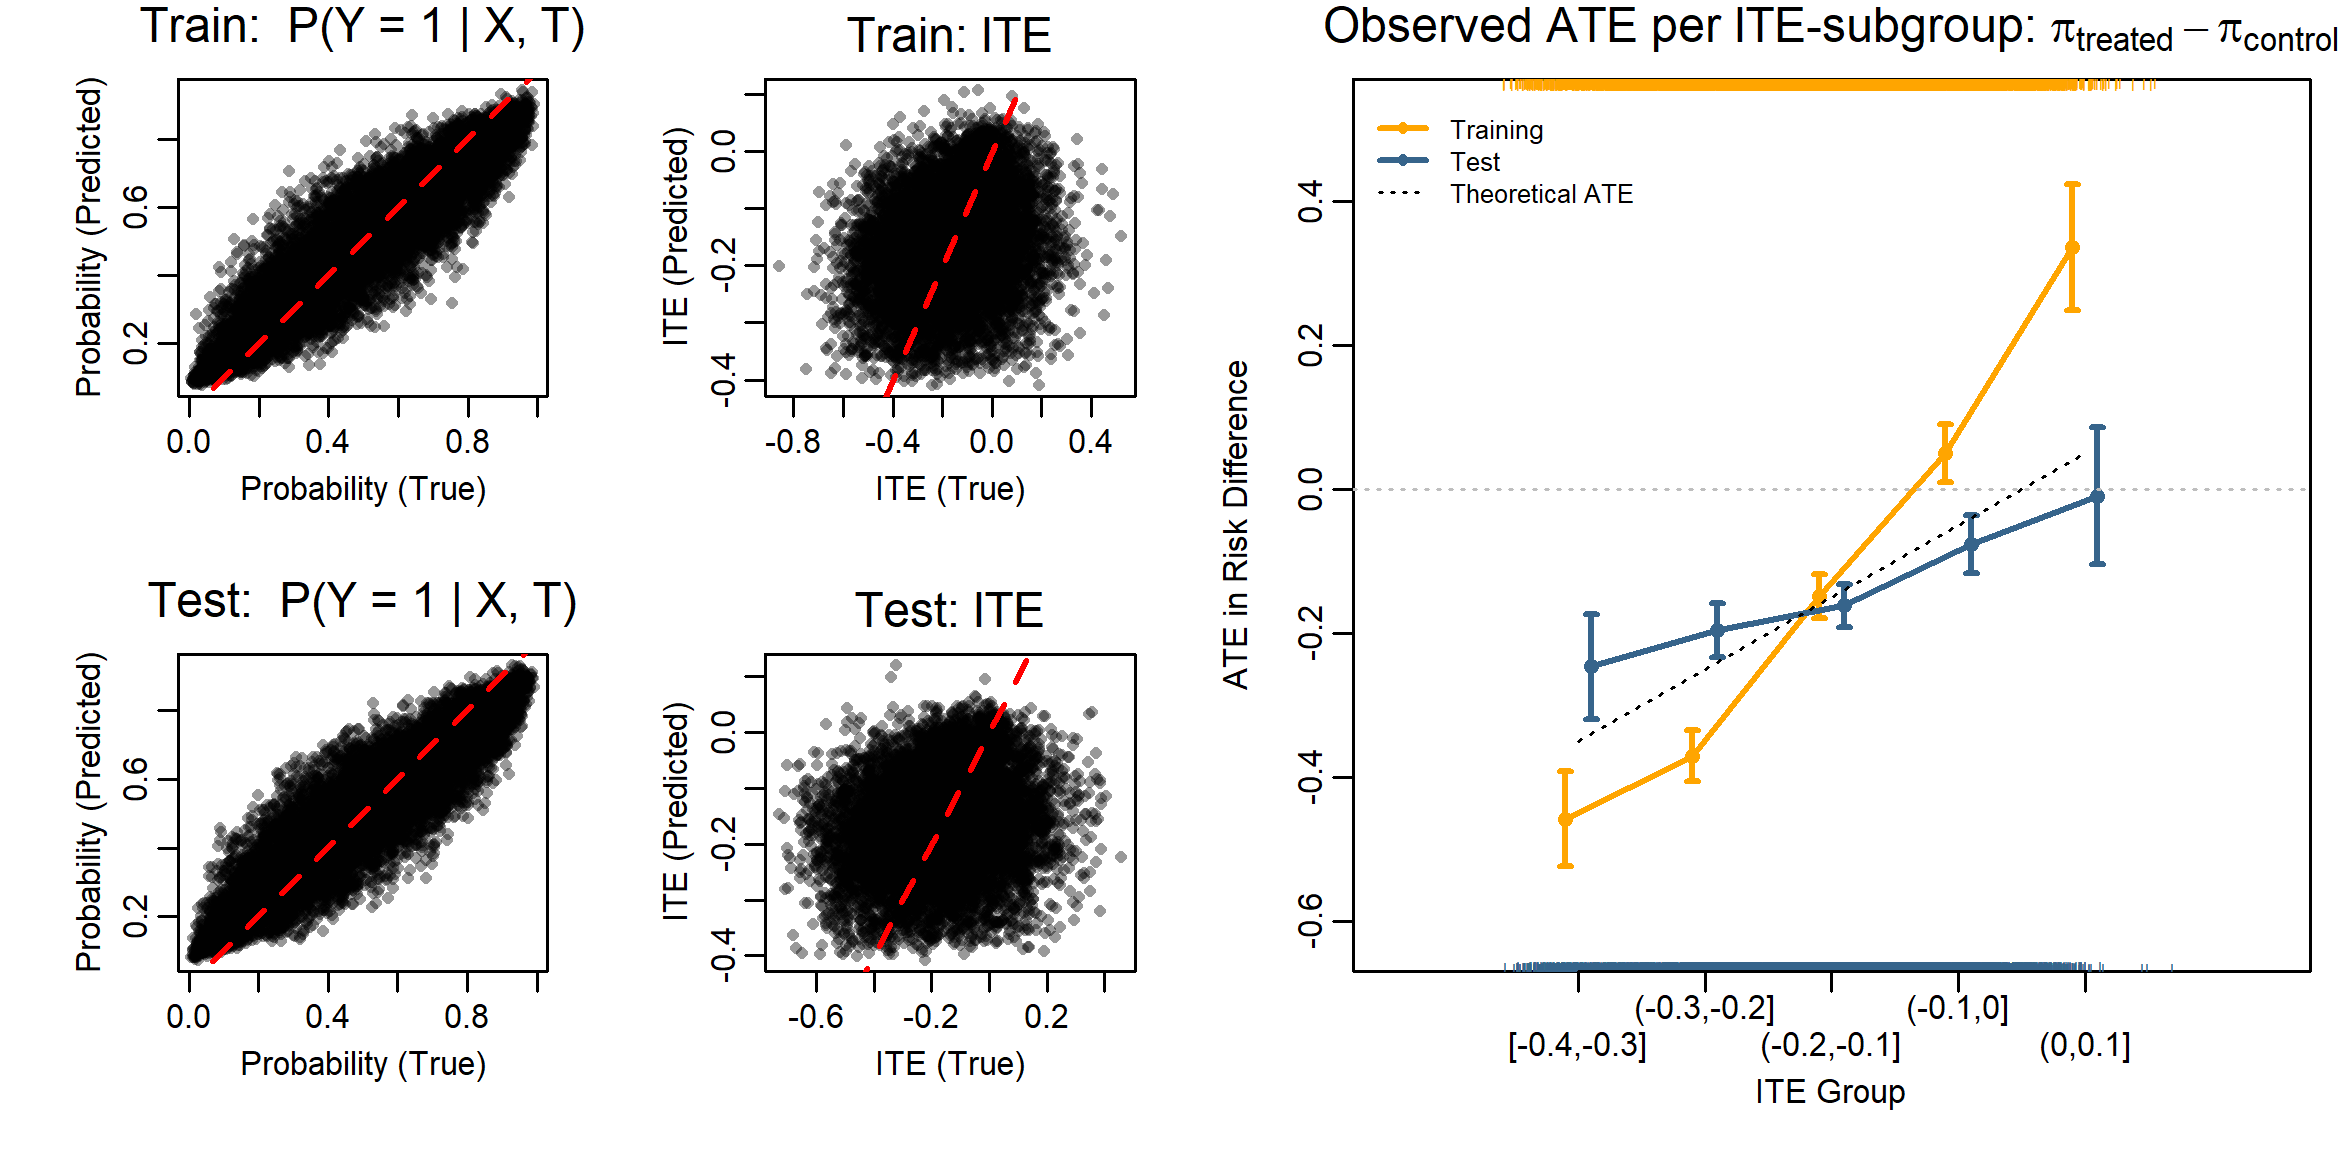
\includegraphics[width=0.9\textwidth]{img/results_ITE_simulation/unobserved_interaction_tuned_rf_tlearner.png}
\caption{Results of the T-learner tuned random forest in Scenario~(2), where there are strong treatment and interaction effects, but variable $X_1$ is not observed. Left: true vs. predicted probabilities for $\text{P}(Y = 1 \mid X, T)$; Middle: true vs. predicted ITEs; Right: observed ATE in terms of risk difference per estimated ITE subgroup.}
\label{fig:unobserved_interaction_tuned_rf_tlearner}
\end{figure}


\clearpage

\subsection{Scenario (3): Fully observed, small effects}

\begin{figure}[htbp]
\centering
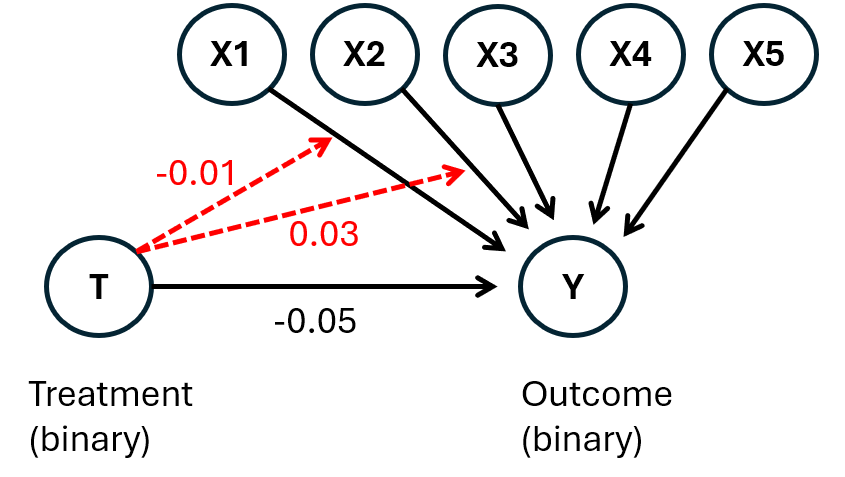
\includegraphics[width=0.35\textwidth]{img/results_ITE_simulation/simulation_small_effects.png}
\caption{DAG for Scenario~(3), where all variables are observed and both treatment and interaction effects are weak. This DAG was previously shown in Figure~\ref{fig:simulation_dags} and is re-plotted here for convenience. The numbers indicate the coefficients on the log-odds scale. Red arrows represent interaction effects between treatment ($T$) and covariates ($X_1$ and $X_2$) on the outcome ($Y$).}
\label{fig:small_interaction_dag}
\end{figure}




\begin{figure}[htbp]
\centering
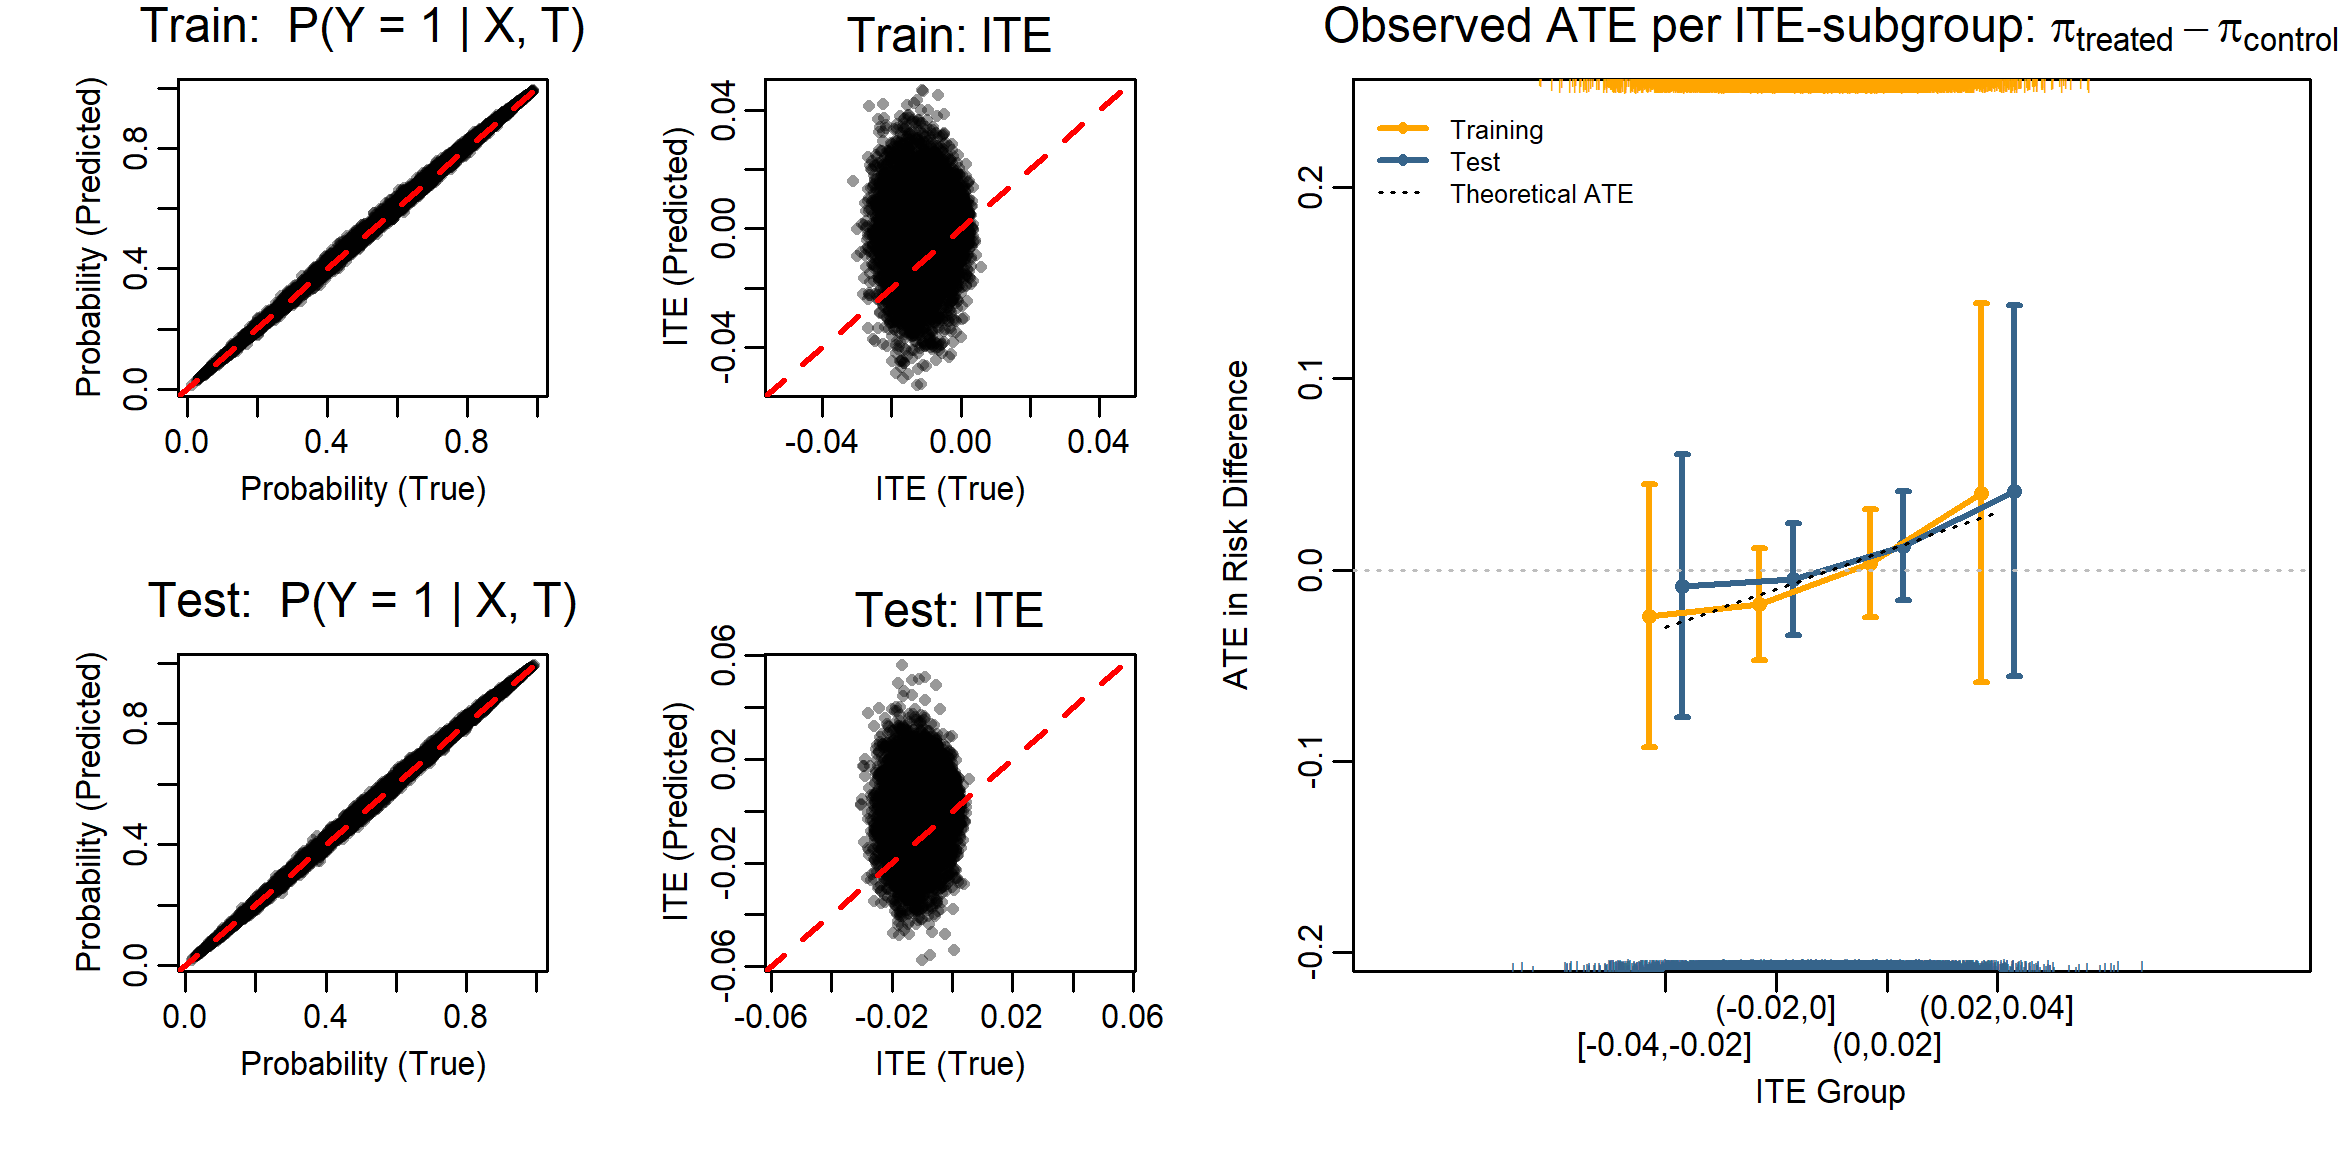
\includegraphics[width=0.9\textwidth]{img/results_ITE_simulation/small_interaction_glm_tlearner.png}
\caption{Results of the T-learner logistic regression in Scenario~(3), where the DAG is fully observed and both treatment and interaction effects are weak. Left: true vs. predicted probabilities for $\text{P}(Y = 1 \mid X, T)$; Middle: true vs. predicted ITEs; Right: observed ATE in terms of risk difference per estimated ITE subgroup.}
\label{fig:small_interaction_glm_tlearner}
\end{figure}




\begin{figure}[htbp]
\centering
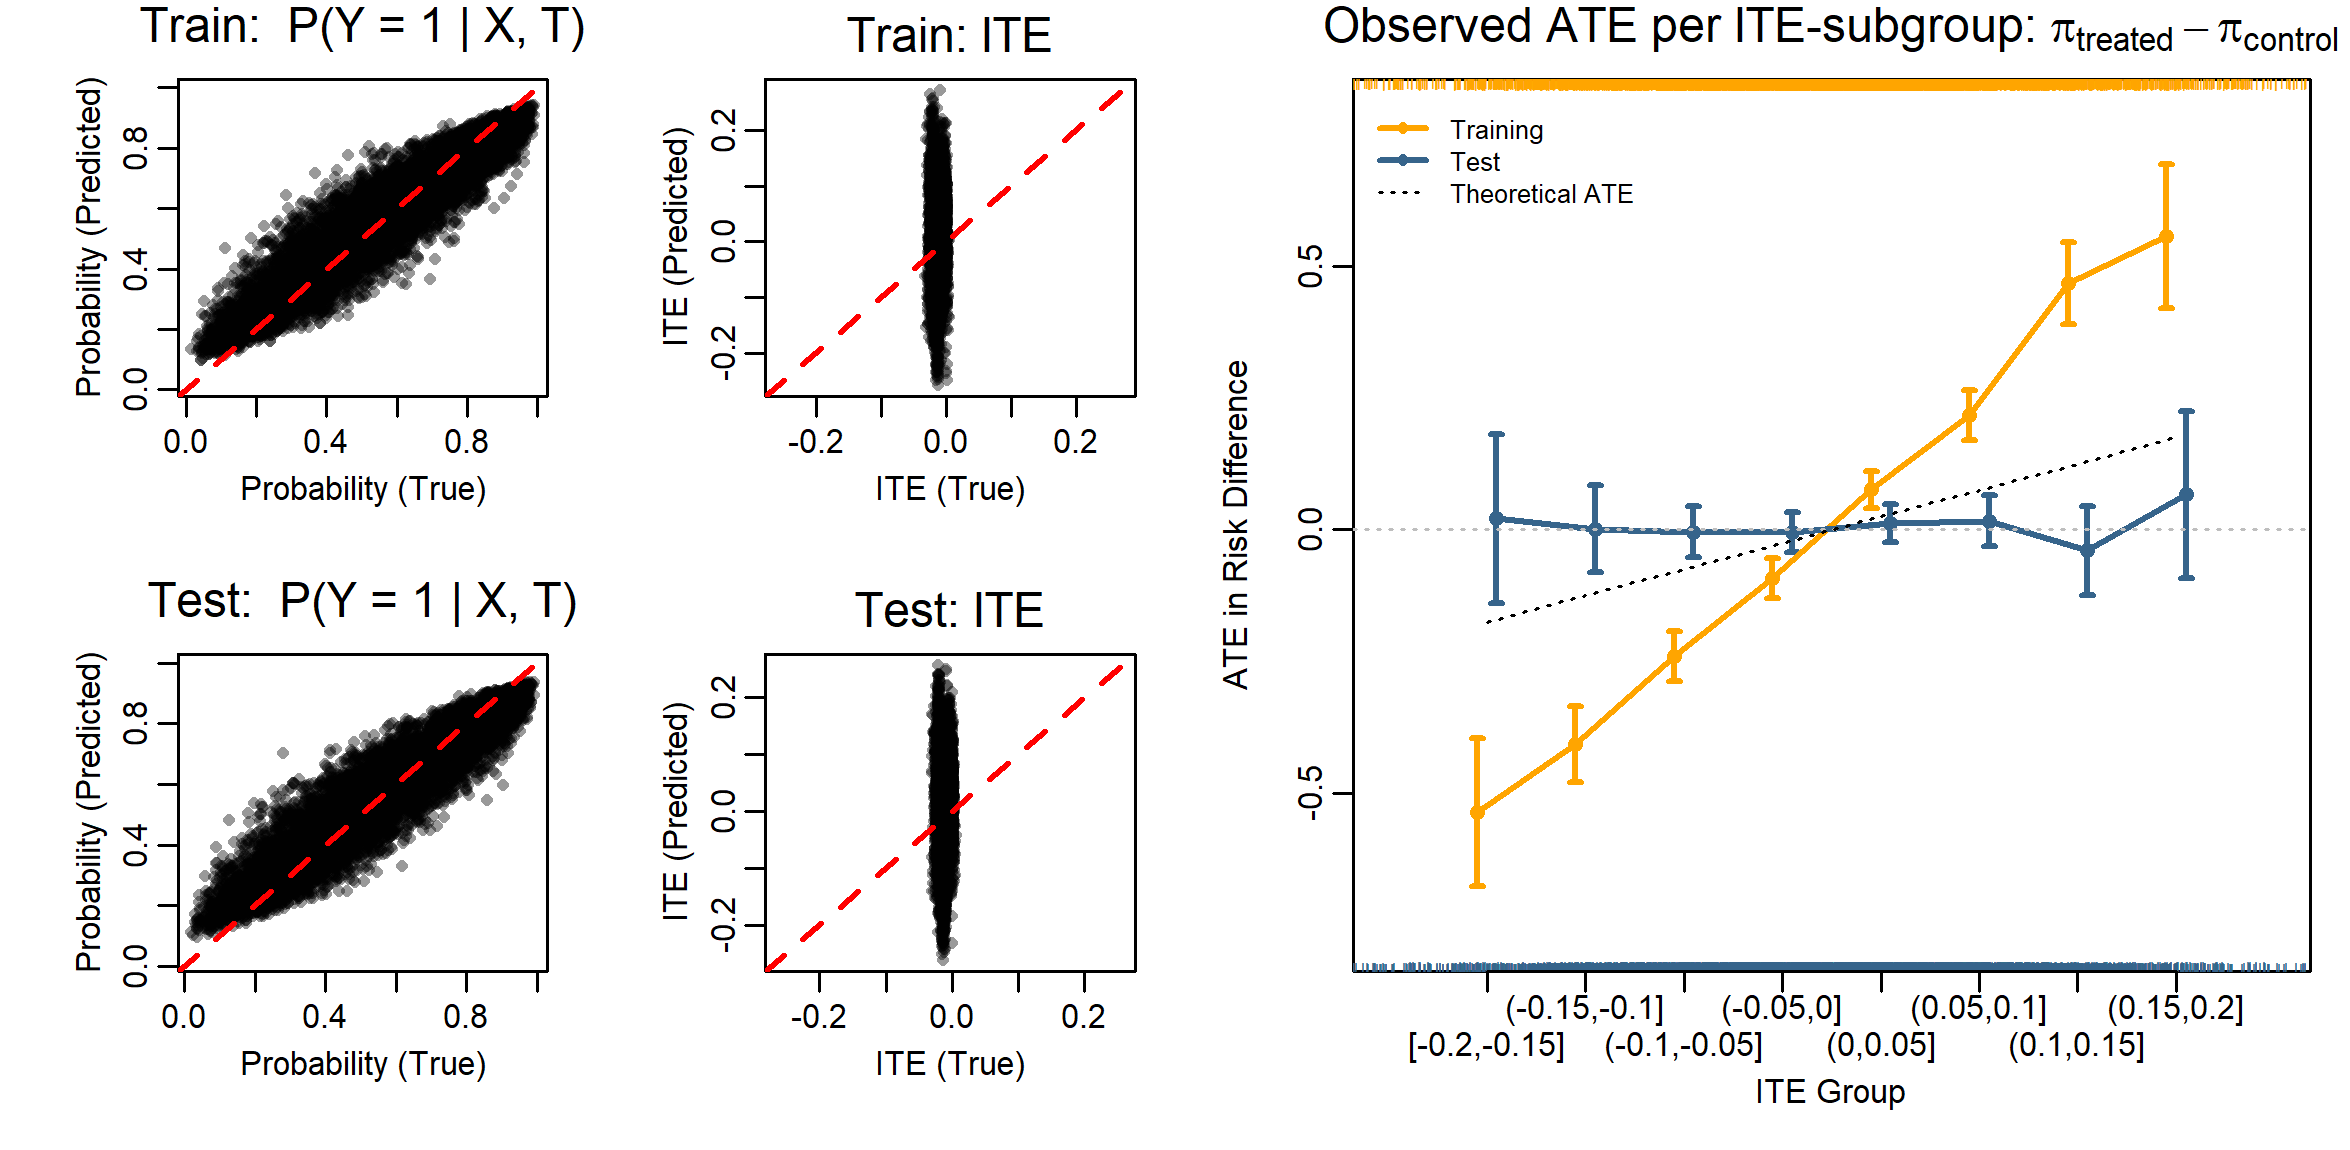
\includegraphics[width=0.9\textwidth]{img/results_ITE_simulation/small_interaction_tuned_rf_tlearner.png}
\caption{Results of the T-learner tuned random forest in Scenario~(3), where the DAG is fully observed and both treatment and interaction effects are weak. Left: true vs. predicted probabilities for $\text{P}(Y = 1 \mid X, T)$; Middle: true vs. predicted ITEs; Right: observed ATE in terms of risk difference per estimated ITE subgroup.}
\label{fig:small_interaction_tuned_rf_tlearner}
\end{figure}


% enforce that starts after all floats have been displayed
\FloatBarrier




\section{Discussion} \label{sec:disc_experiment3}



In Scenario~1, where treatment effect heterogeneity was large and all covariates were observed, the T-learner logistic regression accurately estimated the ITE. The observed ATE, conditional on the respective ITE subgroup, was well calibrated in both the training and test datasets, as shown in the ITE-ATE plot in Figure~\ref{fig:fully_observed_glm_tlearner}. This is as expected, since the data were generated with the same model class (logistic regression), and applying logistic regression as a T-learner for ITE estimation can accurately capture the interaction effects.

The tuned random forest model also performed well. As illustrated in Figure~\ref{fig:fully_tuned_rf_tlearner}, choosing a different model class than that used in the DGP may lead to worse prediction accuracy in terms of $\text{P}(Y = 1 \mid X, T)$ and ITE. This difference between the two models arises because the logistic regression model has only a small number of parameters, and with sufficient data, these parameters can converge to their true values as used in the logistic DGP, allowing near-perfect recovery of the true probabilities and thus ITEs. In contrast, the non-parametric random forest must infer the underlying probabilities from the observed binary outcomes (0 or 1), which are themselves realizations of a Bernoulli process. This introduces inherent noise, making it harder for the model to estimate the true risk accurately -- even with large sample sizes. Nonetheless, the tuned random forest also captured the general trend of the ITEs, as reflected in the ITE-ATE plot, Figure~\ref{fig:fully_tuned_rf_tlearner}. Both models were able to capture treatment effect heterogeneity well under full observability of covariates.



In contrast, the default random forest (i.e., without hyperparameter tuning) performed worse than its tuned counterpart (see Appendix~\ref{sec:default_rf_ite}). As shown in the corresponding ITE-ATE plot, Figure~\ref{fig:fully_observed_rf}, the model exhibited poor calibration and inaccurate ITE estimates, highlighting the importance of proper tuning to ensure reliable ITE estimation and avoid overfitting.


\medskip


\medskip


In Scenario~2, where treatment effect heterogeneity remained large but one important interaction covariate ($X_1$) was not observed, prediction accuracy decreased for both models, and the estimated heterogeneity in terms of the ITE was smaller than the true heterogeneity. Although not all heterogeneity could be recovered, the T-learner logistic regression still estimated the ITEs in the correct direction. As shown in Figure~\ref{fig:unobserved_interaction_glm_tlearner}, the confidence intervals for the ATE per ITE subgroup covered the calibration line. This indicates that individuals estimated to have a smaller ITE indeed experienced worse outcomes under treatment compared to untreated individuals in the same subgroup. Although a considerable number of individuals had a true ITE that was positive, the T-learner logistic regression did not predict a single positive ITE. This shows that the missing covariate $X_1$ prevents detection of individuals who would actually benefit from the treatment. 

In contrast, the T-learner tuned random forest estimated larger treatment effect heterogeneity than the logistic model, but still could not accurately estimate the ITE and also failed to detect patients who would benefit from the treatment. The ITE-ATE plot in Figure~\ref{fig:unobserved_interaction_tuned_rf_tlearner} illustrates that the model discriminates too strongly in the training set and does not generalize well to the test set.


% This is likely due to the fact that the tuned random forest model is a non-parametric model that tries to fit the data as closely as possible, which can lead to overfitting when crucial variables are missing.
\medskip


In Scenario~3, where the true treatment effect heterogeneity was small and all covariates were observed, the T-learner logistic regression estimated a larger heterogeneity than actually present. In the ITE-ATE plot in Figure~\ref{fig:small_interaction_glm_tlearner}, the confidence intervals of all ITE subgroups overlap and include the zero line, indicating that the treatment effect is not significantly different from zero. This matches expectations given the small true effect sizes.

However, the T-learner tuned random forest model incorrectly estimated even larger treatment effect heterogeneity than the logistic regression model. As shown in Figure~\ref{fig:small_interaction_tuned_rf_tlearner}, the model exhibited strong discrimination in the training set but did not to replicate this pattern in the test set, where -- regardless of the estimated ITE -- the observed outcomes in the subgroups were similar.


\medskip


Tuning more flexible models like random forests using cross-validation improved generalization to the test set but led to poor calibration in terms of predicted probabilities vs. empirically observed outcomes in the training set. An illustrative case is shown in Appendix~\ref{sec:calibration_tuned_rf} for the T-learner tuned random forest in Scenario~3 (with weak effects), where calibration was poor in the training set but aligned well with the identity line in the test set. We repeatedly observed this pattern in the tuned random forest when, in the ITE-ATE plot, results from the training set did not generalize to the test set. This highlights the importance of evaluating models on an independent test set, when tuning a model to prevent overfitting. Although, evaluation on a test set should be done in any case.

\medskip

In this experiment, we showed that even when causal ML models for ITE estimation are well calibrated in terms of prediction accuracy $\text{P}(Y = 1 \mid \mathbf{X}, T)$, they can still fail to estimate the ITE accurately under less favorable scenarios. In cases of full observability of covariates but low interaction effects, models may estimate too high heterogeneity that is not present in the data. However, this can become visible in the ITE-ATE plot on the test set, which reveals that the apparent heterogeneity does not generalize. 
But we also observed that when important effect-modifying covariates are missing, the models may fail to detect treatment effect heterogeneity altogether, as shown in Scenario~2. In such cases, the estimated ITEs may be too small or even negative, suggesting that the model does not capture the true treatment effect heterogeneity. This makes it difficult to distinguish between a true lack of heterogeneity and the failure to capture it due to unobserved effect modifiers.


\citet{vegetabile2021} also analyzed the effect of unobserved interaction variables. He pointed out that as long as all confounding variables $\mathbf{X}$ are observed and conditioned on, the ignorability assumption required for ITE estimation is satisfied -- even in the presence of an unobserved interaction variable $Z$. However, if such a variable $Z$ exists, the estimated ITEs would be biased, and this issue could arise even in an RCT setting where confounding is removed through randomization.

\citet{nichols2007} discusses various methods for estimating causal effects from observational data, including in the presence of unobserved variables. One of these methods, instrumental variables (IV), can help reduce bias from unobserved confounding. Whether IV methods can also address unobserved effect modifiers in the context of ITE estimation is not something we explored, and remains beyond the scope of this thesis.



% such as the use of instrumental variables (IV) to estimate CATE in the presence of unobserved confounders \citep{nichols2007, hartford2017}. \citet{frauen2023} propose a model based on IV that is said to also be applicable on observational data. However, this is not yet widely adopted and remains an area for future research.

 % check more details, they also have an example DAG, however it is not yet accepted and still under review






